\documentclass[12pt,a4paper]{article}
\usepackage[utf8]{inputenc}
\usepackage[french]{babel}
\usepackage[T1]{fontenc}
\usepackage{amsmath}
\usepackage{amsfonts}
\usepackage{amssymb}
\usepackage{graphicx}
\usepackage{fourier}
\usepackage{caption} 
\usepackage{subcaption}
\usepackage{float}% importtant pour mettre les images sans espaces autour.
\captionsetup{font=small}
\usepackage[left=2cm,right=2cm,top=2cm,bottom=2cm]{geometry}
\title{Compte rendu du TP5 : Magnétostatique}
\author{BATHILY Ousmane \\ Universite Paris-Saclay}
\date{}
\begin{document}
\renewcommand{\tablename}{Tableau}

\maketitle
\section{Introduction}
L'objectif de ce TP est de faire l'étude de plusieurs dispositifs nous permettant d'obtenir un champ magnétique quasiment uniforme (montage de Helmholtz), en utilisant tout d'abord une puis ensuite deux  bobines montées en série et parcourues par un courant constant $I$ créant ainsi un champ $\vec{B}$.
\section{Champ magnétique généré par une seule bobine}
Dans cette première partie, nous allons généré un champ à l'aide d'une bobine étant parcourue par un courant d'intensité $I$.\\
Voici la liste du matériel dont nous allons avoir besoin :\\
\\4
- Une bobine de rayon moyen $R$ = 20 $cm$, comportant $n$ = 154 spires dont la resistance interne vaut 2,2 $\Omega$.\\
- Un multimètre que nous brancherons en série dans le circuit.\\
- Une genérateur de courant continu.\\
- Une règle fixée sur la table.\\
- Un Teslamètre, qui nous servira à mesurer l'intensité du champ $\vec{B}$ donnée en ($mT$).\\
- Une boussole permettant de nous donner l'orientation de $\vec{B}$.\\
\\
Voici maintenant un schéma du circuit que nous allons réaliser : \\
\begin{figure}[H]
\begin{center}
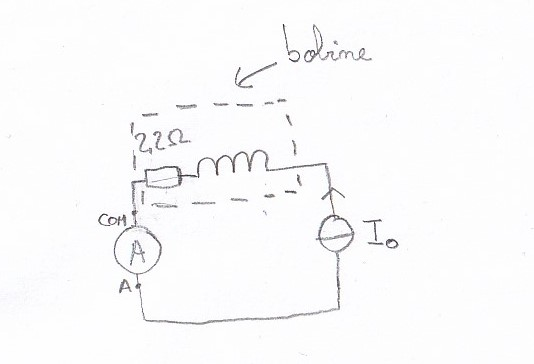
\includegraphics[scale=1]{circuit1.jpg}   
\caption{Schéma du premier montage}
\end{center}
\end{figure}
En réglant l'alimentation de sorte à ce qu'elle fournisse un courant de 2$A$, on remarque que la boussole est orientée selon l'axe perpendiculaire au centre de la bobine. Concernant son sens, la boussole nous indique le Nord en tout point de cet axe. Voici à quoi ressemble qualitativement les lignes de champ : \\
\begin{figure}[H]
\begin{center}
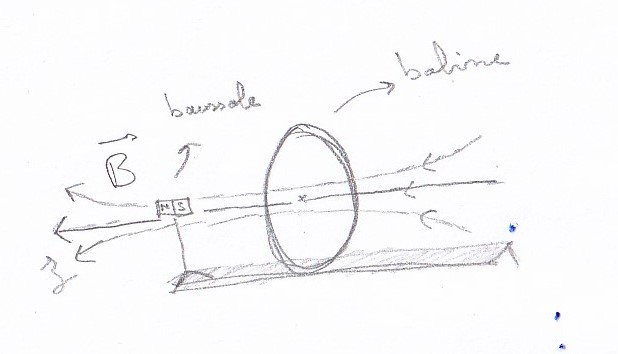
\includegraphics[scale=1]{ldc.jpg}   
\caption{Lignes de champ de $\vec{B}$, avec le montage en figure (1)}
\end{center}
\end{figure}
En inversant ensuite le sens de circulation du courant, on remarque que les lignes de champ sont maintenant de sens opposées, traduisant le fait que $\vec{B}$ soit proportionnel à $I$.\\
\\Nous allons maintenant effectuer une série de mesures, celle de l'intensité du champ magnétique crée par la bobine, soumise à un courant de $2A$ en utilisant la sonde qui est placée à une certaine distance $z$ du centre de la bobine, distance pouvant être mesurée à l'aide de la règle graduée mise à notre disposition. Voici un schéma de l'expérience : \\
\begin{figure}[H]
\begin{center}
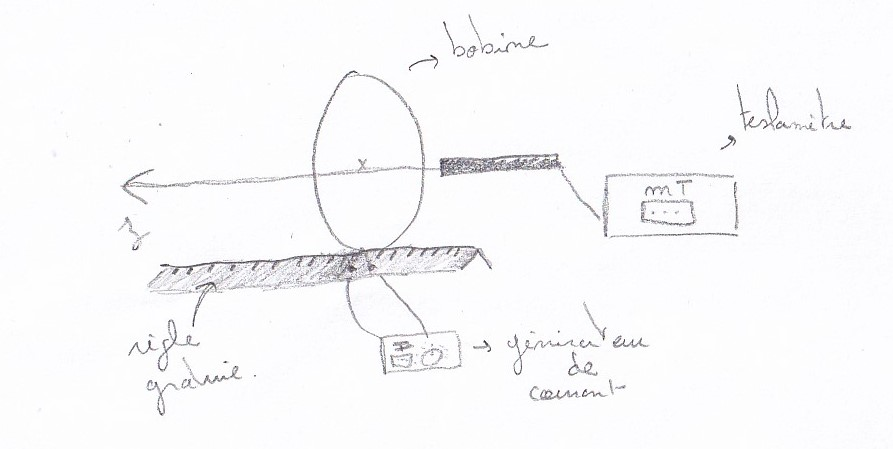
\includegraphics[scale=1]{exp1.jpg}   
\caption{Schéma de l'expérience}
\end{center}
\end{figure}
Voici les valeurs obtenues, sachant que l'incertidude sur la sonde de Hall vaut $5\cdot10^{-2} mT$ et celle de la règle graduée un demi millimètre.
\begin{table}[H]
\begin{center}
\begin{tabular}{|c|c|}
\hline
$z \pm 5\cdot10^{-4} (m)$ & $B\pm 5\cdot10^{-2} (mT)$\\ 
\hline
-20 & 0.27 \\
\hline
-15 & 0.42 \\
\hline
-10 & 0.62 \\
\hline
-5 & 0.82\\
\hline
0 & 0.91\\
\hline
5 & 0.81\\
\hline
10 & 0.61\\
\hline
15 & 0.42\\
\hline
20 & 0.27\\
\hline
25 & 0.16\\
\hline
30 & 0.09\\
\hline
\end{tabular}
\caption{Intensité du champ magnétique $B$ en fonction de la distance $z$ de la sonde par rapport au centre de la bobine.}
\end{center}
\end{table}
On remarque, au premier coup d'œil une symétrie entre les valeurs de B avant et après $z$ = 0 cm. Le champ magnétique décroit evidemment avec la distance mais $B$ serait-il, comme le champ électrique inversement proportionnel au carré de la distance ?\\
Voici l'ensemble des points obtenus représentés sur un graphique :\\
\begin{figure}[H]
\begin{center}
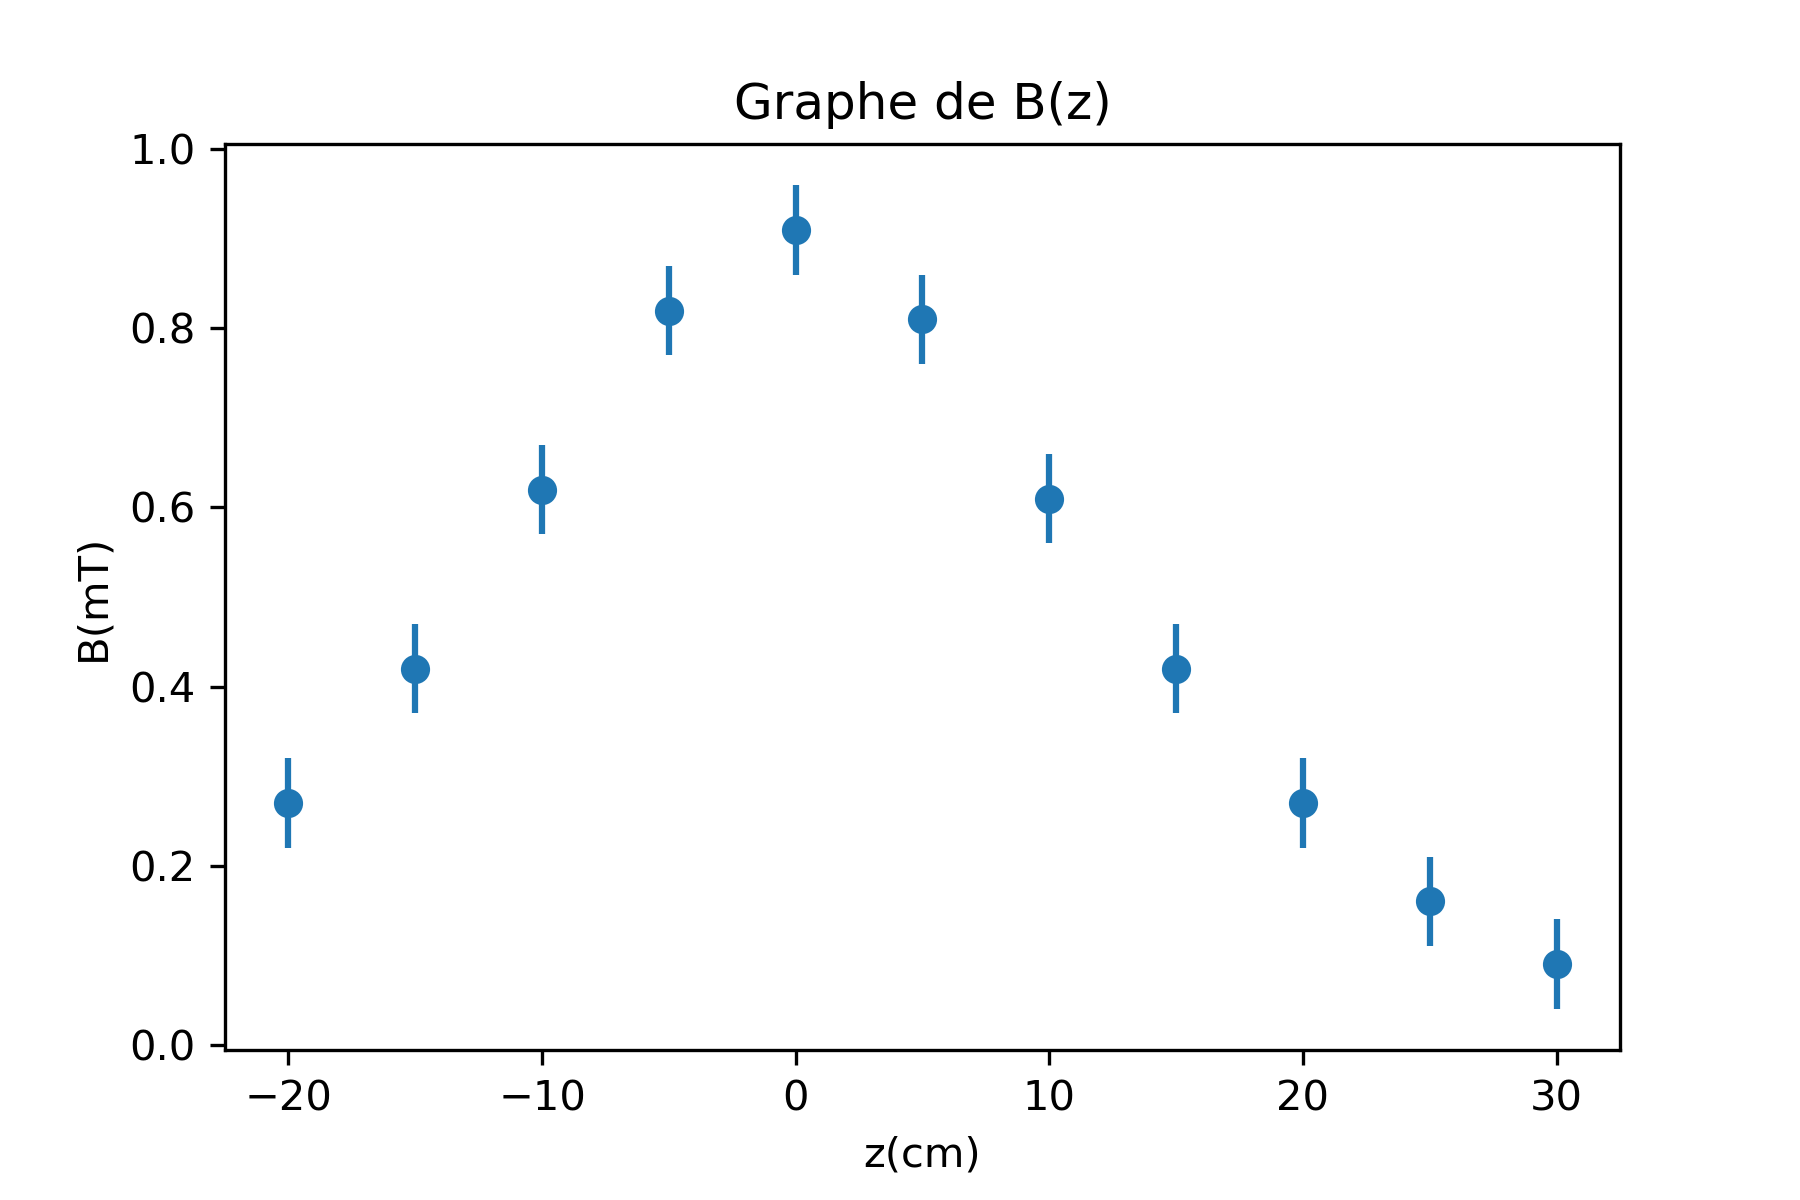
\includegraphics[scale=1]{bz.png}
\caption{Graphe de B en fonction de z dont le maximum est à $z = 0$ $cm$.}
\end{center}
\end{figure}

D'après la loi de Biot-Savart et en nous plaçant dans le cas d'une bobine de $n$ spires de rayon $R$ et parcourue d'un courant I, le champ B en un point distant de $z$ par rapport au centre de la bobine est donné par la relation:
\begin{equation}
B(z) = \frac{\mu_{0}In}{2R}\sin^3(\alpha) \text{, avec $\mu_0 = 4\pi\cdot10^{-7} SI$}
\end{equation}
\begin{figure}[H]
\centering
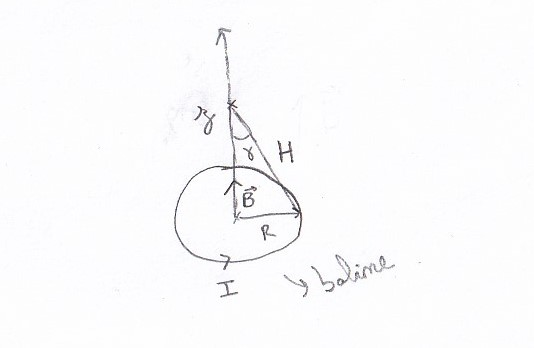
\includegraphics[scale=1]{s1.jpg}
\caption{Schéma illustrant l'équation (1)}

\end{figure}

Sachant que $\sin(\alpha) = \frac{R}{H}$ et que $H^2=z^2+R^2$ on en déduit que :
\begin{equation}
\sin^3(\alpha) = \frac{R^3}{\sqrt{z^2+R^2}^3}
\end{equation}
\begin{equation}
\Longleftrightarrow B(z) = \frac{\mu_{0}In}{2R}\frac{R^3}{\sqrt{z^2+R^2}^3}
\end{equation}
\begin{equation}
\Longleftrightarrow B(z) = \frac{\mu_{0}InR^2}{2(z^2+R^2)^{3/2}}
\end{equation}
\begin{equation}
\text{, avec : } B_0 = \frac{\mu_0In}{2R} = 9,67\cdot10^{-4} T
\end{equation}
\\
On remarque que finalement $B\varpropto\frac{1}{z^3}$ . Ajoutons maintenant à la figure précédente le graphe de $B(z)$.
\begin{figure}[H]
\begin{center}
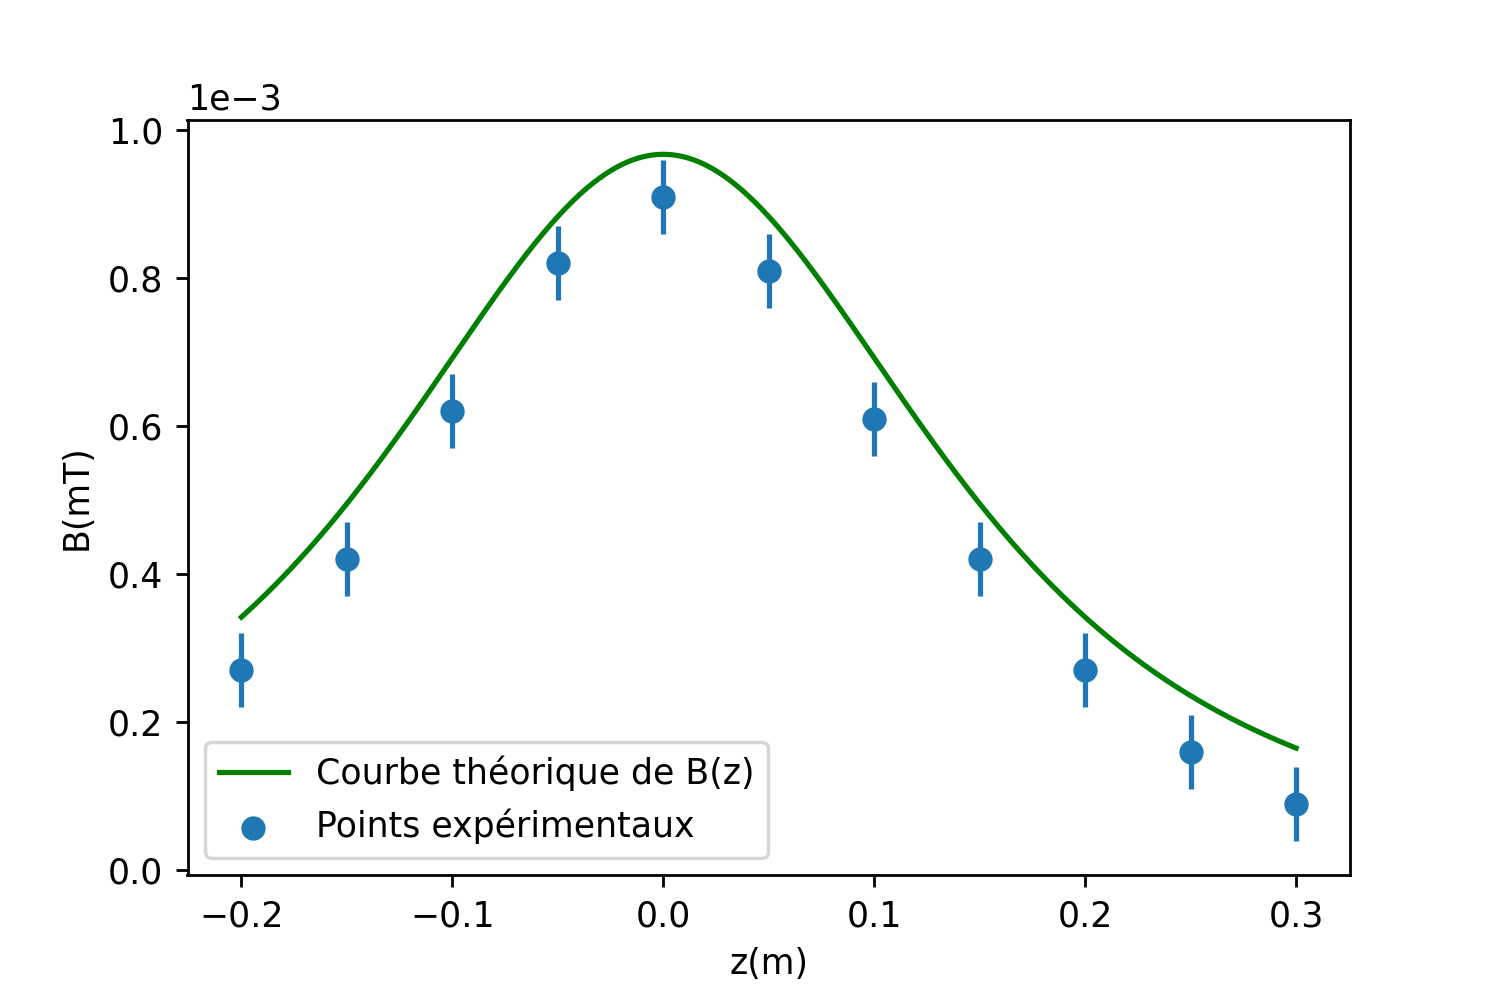
\includegraphics[scale=0.8]{c1.png}
\caption{Comparaison des données expérimentales et de la courbe théorique de B(z)}
\end{center}
\end{figure}
La courbe théorique est toujours au dessus de nos points expérimentaux en étant très proche de la valeur maximale en prenant en compte l'incertitude sur $B$, les mesures ont l'air d'avoir bien été effectuées.
Nous allons maintenant comparer comme précédemment l'intensité du champ $B$ mais cette fois en fonction du courant I avec $z$ = 0 cm.\\
D'après l'équation (5), on a :
\begin{equation}
B_0(I) = \frac{\mu_0In}{2R}
\end{equation}
La relation est donc linéaire, nous allons vérifier cela en effectuant une série de mesures et voici ce que nous obtenons :
\begin{table}[H]
\begin{center}
\begin{tabular}{|c|c|}
\hline
$I \pm 5\cdot10^{-4} (A)$ & $B\pm 5\cdot10^{-2} (mT)$\\ 
\hline
2.001 & 0.92 \\
\hline
1.801 & 0.81 \\
\hline
1.600 & 0.72 \\
\hline
1.398 & 0.62\\
\hline
1.220 & 0.55\\
\hline
1.000 & 0.44\\
\hline
0.840 & 0.34\\
\hline
0.598 & 0.25\\
\hline
0.400 & 0.14\\
\hline
0.200 & 0.04\\
\hline
\end{tabular}
\caption{Intensité du champ magnétique $B$ en fonction du courant I}
\end{center}
\end{table}
\begin{figure}[H]
\begin{center}
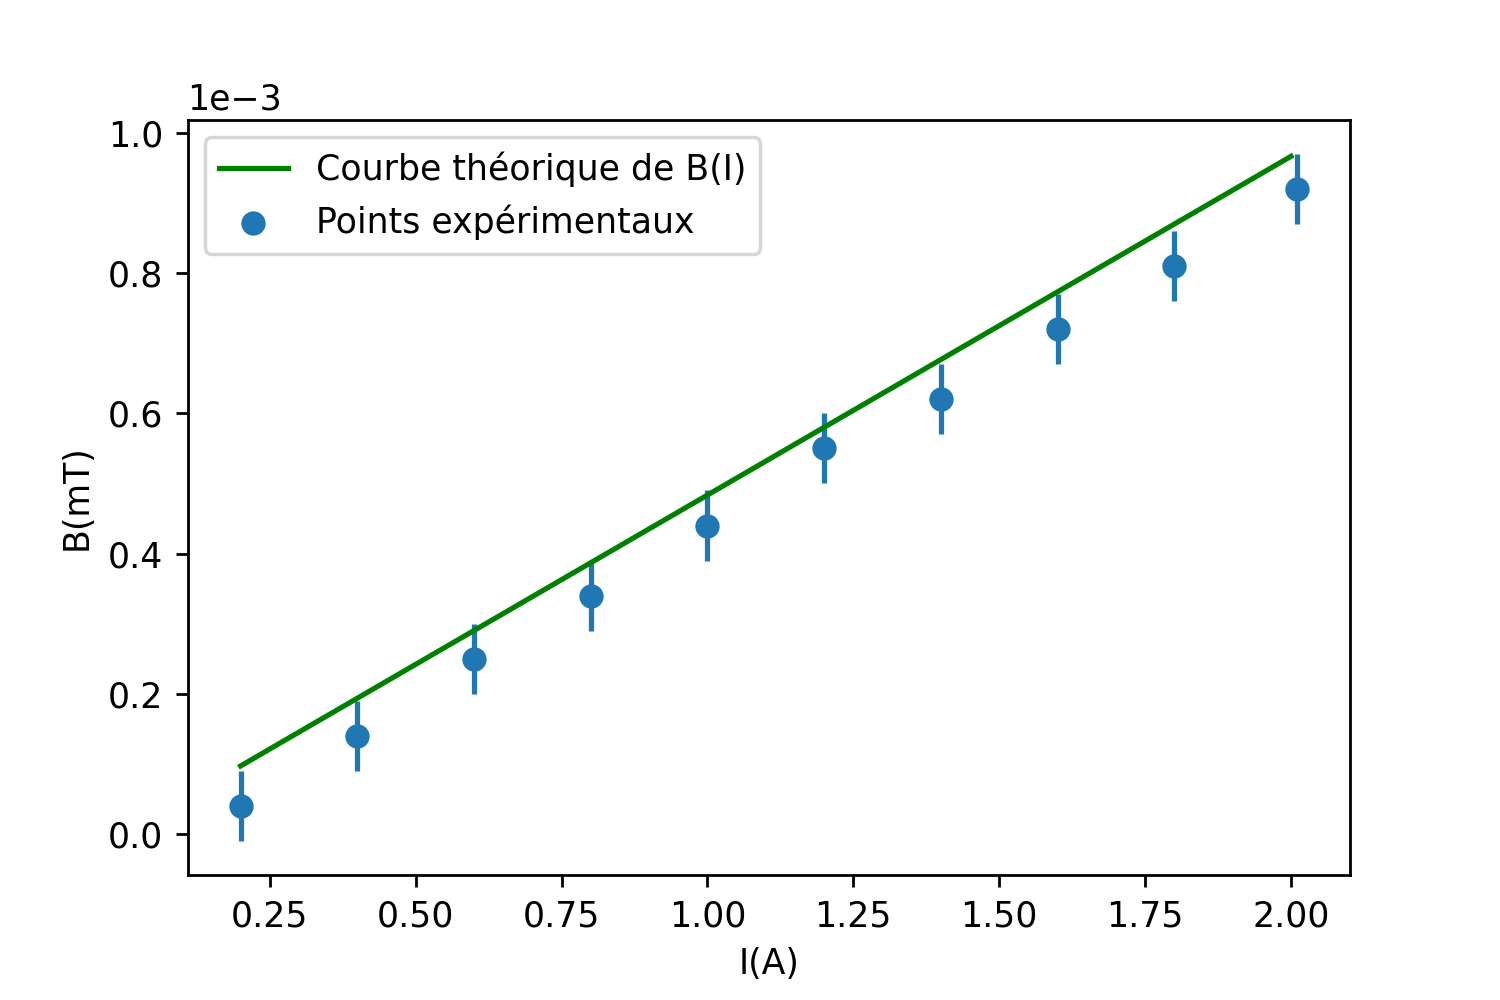
\includegraphics[scale=1]{c2.png}
\caption{Comparaison des données expérimentales et de la courbe théorique de $B(I)$}
\end{center}
\end{figure}
Les données sont encore une fois bien en accord avec la loi de Boit-Savart, ce qui est rassurant.
\end{document}